\documentclass[twoside]{book}

% Packages required by doxygen
\usepackage{fixltx2e}
\usepackage{calc}
\usepackage{doxygen}
\usepackage{graphicx}
\usepackage[utf8]{inputenc}
\usepackage{makeidx}
\usepackage{multicol}
\usepackage{multirow}
\PassOptionsToPackage{warn}{textcomp}
\usepackage{textcomp}
\usepackage[nointegrals]{wasysym}
\usepackage[table]{xcolor}

% Font selection
\usepackage[T1]{fontenc}
\usepackage{mathptmx}
\usepackage[scaled=.90]{helvet}
\usepackage{courier}
\usepackage{amssymb}
\usepackage{sectsty}
\renewcommand{\familydefault}{\sfdefault}
\allsectionsfont{%
  \fontseries{bc}\selectfont%
  \color{darkgray}%
}
\renewcommand{\DoxyLabelFont}{%
  \fontseries{bc}\selectfont%
  \color{darkgray}%
}
\newcommand{\+}{\discretionary{\mbox{\scriptsize$\hookleftarrow$}}{}{}}

% Page & text layout
\usepackage{geometry}
\geometry{%
  a4paper,%
  top=2.5cm,%
  bottom=2.5cm,%
  left=2.5cm,%
  right=2.5cm%
}
\tolerance=750
\hfuzz=15pt
\hbadness=750
\setlength{\emergencystretch}{15pt}
\setlength{\parindent}{0cm}
\setlength{\parskip}{0.2cm}
\makeatletter
\renewcommand{\paragraph}{%
  \@startsection{paragraph}{4}{0ex}{-1.0ex}{1.0ex}{%
    \normalfont\normalsize\bfseries\SS@parafont%
  }%
}
\renewcommand{\subparagraph}{%
  \@startsection{subparagraph}{5}{0ex}{-1.0ex}{1.0ex}{%
    \normalfont\normalsize\bfseries\SS@subparafont%
  }%
}
\makeatother

% Headers & footers
\usepackage{fancyhdr}
\pagestyle{fancyplain}
\fancyhead[LE]{\fancyplain{}{\bfseries\thepage}}
\fancyhead[CE]{\fancyplain{}{}}
\fancyhead[RE]{\fancyplain{}{\bfseries\leftmark}}
\fancyhead[LO]{\fancyplain{}{\bfseries\rightmark}}
\fancyhead[CO]{\fancyplain{}{}}
\fancyhead[RO]{\fancyplain{}{\bfseries\thepage}}
\fancyfoot[LE]{\fancyplain{}{}}
\fancyfoot[CE]{\fancyplain{}{}}
\fancyfoot[RE]{\fancyplain{}{\bfseries\scriptsize Generated on Mon Jan 4 2016 15\+:01\+:21 for Module\+Calibration by Doxygen }}
\fancyfoot[LO]{\fancyplain{}{\bfseries\scriptsize Generated on Mon Jan 4 2016 15\+:01\+:21 for Module\+Calibration by Doxygen }}
\fancyfoot[CO]{\fancyplain{}{}}
\fancyfoot[RO]{\fancyplain{}{}}
\renewcommand{\footrulewidth}{0.4pt}
\renewcommand{\chaptermark}[1]{%
  \markboth{#1}{}%
}
\renewcommand{\sectionmark}[1]{%
  \markright{\thesection\ #1}%
}

% Indices & bibliography
\usepackage{natbib}
\usepackage[titles]{tocloft}
\setcounter{tocdepth}{3}
\setcounter{secnumdepth}{5}
\makeindex

% Hyperlinks (required, but should be loaded last)
\usepackage{ifpdf}
\ifpdf
  \usepackage[pdftex,pagebackref=true]{hyperref}
\else
  \usepackage[ps2pdf,pagebackref=true]{hyperref}
\fi
\hypersetup{%
  colorlinks=true,%
  linkcolor=blue,%
  citecolor=blue,%
  unicode%
}

% Custom commands
\newcommand{\clearemptydoublepage}{%
  \newpage{\pagestyle{empty}\cleardoublepage}%
}


%===== C O N T E N T S =====

\begin{document}

% Titlepage & ToC
\hypersetup{pageanchor=false,
             bookmarks=true,
             bookmarksnumbered=true,
             pdfencoding=unicode
            }
\pagenumbering{roman}
\begin{titlepage}
\vspace*{7cm}
\begin{center}%
{\Large Module\+Calibration }\\
\vspace*{1cm}
{\large Generated by Doxygen 1.8.7}\\
\vspace*{0.5cm}
{\small Mon Jan 4 2016 15:01:21}\\
\end{center}
\end{titlepage}
\clearemptydoublepage
\tableofcontents
\clearemptydoublepage
\pagenumbering{arabic}
\hypersetup{pageanchor=true}

%--- Begin generated contents ---
\chapter{Hierarchical Index}
\section{Class Hierarchy}
This inheritance list is sorted roughly, but not completely, alphabetically\+:\begin{DoxyCompactList}
\item \contentsline{section}{Config\+File}{\pageref{classConfigFile}}{}
\item \contentsline{section}{Element}{\pageref{classElement}}{}
\begin{DoxyCompactList}
\item \contentsline{section}{Crystal}{\pageref{classCrystal}}{}
\item \contentsline{section}{Module}{\pageref{classModule}}{}
\item \contentsline{section}{Mppc}{\pageref{classMppc}}{}
\end{DoxyCompactList}
\item \contentsline{section}{Config\+File\+:\+:file\+\_\+not\+\_\+found}{\pageref{structConfigFile_1_1file__not__found}}{}
\item \contentsline{section}{Input\+File}{\pageref{classInputFile}}{}
\item \contentsline{section}{Config\+File\+:\+:key\+\_\+not\+\_\+found}{\pageref{structConfigFile_1_1key__not__found}}{}
\item \contentsline{section}{Point}{\pageref{structPoint}}{}
\item \contentsline{section}{Config\+File\+:\+:split\+\_\+t}{\pageref{structConfigFile_1_1split__t}}{}
\end{DoxyCompactList}

\chapter{Class Index}
\section{Class List}
Here are the classes, structs, unions and interfaces with brief descriptions\+:\begin{DoxyCompactList}
\item\contentsline{section}{\hyperlink{classConfigFile}{Config\+File} }{\pageref{classConfigFile}}{}
\item\contentsline{section}{\hyperlink{classCrystal}{Crystal} }{\pageref{classCrystal}}{}
\item\contentsline{section}{\hyperlink{classElement}{Element} \\*Base class of the analysis }{\pageref{classElement}}{}
\item\contentsline{section}{\hyperlink{structConfigFile_1_1file__not__found}{Config\+File\+::file\+\_\+not\+\_\+found} }{\pageref{structConfigFile_1_1file__not__found}}{}
\item\contentsline{section}{\hyperlink{classInputFile}{Input\+File} }{\pageref{classInputFile}}{}
\item\contentsline{section}{\hyperlink{structConfigFile_1_1key__not__found}{Config\+File\+::key\+\_\+not\+\_\+found} }{\pageref{structConfigFile_1_1key__not__found}}{}
\item\contentsline{section}{\hyperlink{classModule}{Module} }{\pageref{classModule}}{}
\item\contentsline{section}{\hyperlink{classMppc}{Mppc} }{\pageref{classMppc}}{}
\item\contentsline{section}{\hyperlink{structPoint}{Point} }{\pageref{structPoint}}{}
\item\contentsline{section}{\hyperlink{structConfigFile_1_1split__t}{Config\+File\+::split\+\_\+t} }{\pageref{structConfigFile_1_1split__t}}{}
\end{DoxyCompactList}

\chapter{Class Documentation}
\hypertarget{classConfigFile}{\section{Config\+File Class Reference}
\label{classConfigFile}\index{Config\+File@{Config\+File}}
}


Collaboration diagram for Config\+File\+:
\nopagebreak
\begin{figure}[H]
\begin{center}
\leavevmode
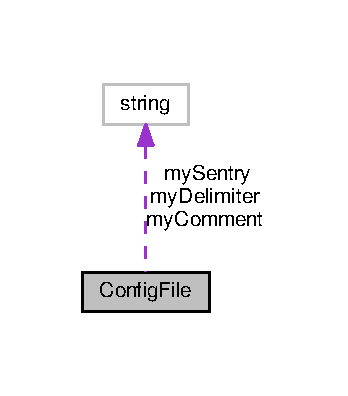
\includegraphics[width=167pt]{classConfigFile__coll__graph}
\end{center}
\end{figure}
\subsection*{Classes}
\begin{DoxyCompactItemize}
\item 
struct \hyperlink{structConfigFile_1_1file__not__found}{file\+\_\+not\+\_\+found}
\item 
struct \hyperlink{structConfigFile_1_1key__not__found}{key\+\_\+not\+\_\+found}
\item 
struct \hyperlink{structConfigFile_1_1split__t}{split\+\_\+t}
\end{DoxyCompactItemize}
\subsection*{Public Member Functions}
\begin{DoxyCompactItemize}
\item 
\hypertarget{classConfigFile_a2690c3c6b72869b65d168791b28264dc}{{\bfseries Config\+File} (string filename, string delimiter=\char`\"{}=\char`\"{}, string comment=\char`\"{}\#\char`\"{}, string sentry=\char`\"{}End\+Config\+File\char`\"{})}\label{classConfigFile_a2690c3c6b72869b65d168791b28264dc}

\item 
\hypertarget{classConfigFile_a3bb52712de11cc22bd8db6fe27711b68}{{\footnotesize template$<$class T $>$ }\\T {\bfseries read} (const string \&key) const }\label{classConfigFile_a3bb52712de11cc22bd8db6fe27711b68}

\item 
\hypertarget{classConfigFile_ae7ca2c239c8a2994c6c9af5060c4a8f1}{{\footnotesize template$<$class T $>$ }\\T {\bfseries read} (const string \&key, const T \&value) const }\label{classConfigFile_ae7ca2c239c8a2994c6c9af5060c4a8f1}

\item 
\hypertarget{classConfigFile_aa726137d059f68e65e88529afdb071f7}{{\footnotesize template$<$class T $>$ }\\bool {\bfseries read\+Into} (T \&var, const string \&key) const }\label{classConfigFile_aa726137d059f68e65e88529afdb071f7}

\item 
\hypertarget{classConfigFile_a0f5a3275ead09adcc7ce5d372b570381}{{\footnotesize template$<$class T $>$ }\\bool {\bfseries read\+Into} (T \&var, const string \&key, const T \&value) const }\label{classConfigFile_a0f5a3275ead09adcc7ce5d372b570381}

\item 
\hypertarget{classConfigFile_ad82a9c27d698a5e805cf5f6f0ad1bfd5}{{\footnotesize template$<$class T $>$ }\\void {\bfseries add} (string key, const T \&value)}\label{classConfigFile_ad82a9c27d698a5e805cf5f6f0ad1bfd5}

\item 
\hypertarget{classConfigFile_afca295f72101b138ad2702a11c342f37}{void {\bfseries remove} (const string \&key)}\label{classConfigFile_afca295f72101b138ad2702a11c342f37}

\item 
\hypertarget{classConfigFile_afd3d1146ae212a7e5802961f5ad3fe91}{bool {\bfseries key\+Exists} (const string \&key) const }\label{classConfigFile_afd3d1146ae212a7e5802961f5ad3fe91}

\item 
\hypertarget{classConfigFile_adcc1df41c7d669a7cc81c47b85b0ee14}{string {\bfseries get\+Delimiter} () const }\label{classConfigFile_adcc1df41c7d669a7cc81c47b85b0ee14}

\item 
\hypertarget{classConfigFile_a2b0cd50789ea83b1a12bf39293c7401a}{string {\bfseries get\+Comment} () const }\label{classConfigFile_a2b0cd50789ea83b1a12bf39293c7401a}

\item 
\hypertarget{classConfigFile_adf270b0cf2a1b034fc18fd2e82296760}{string {\bfseries get\+Sentry} () const }\label{classConfigFile_adf270b0cf2a1b034fc18fd2e82296760}

\item 
\hypertarget{classConfigFile_af28390aba7d8f399ac734c074e659b99}{string {\bfseries set\+Delimiter} (const string \&s)}\label{classConfigFile_af28390aba7d8f399ac734c074e659b99}

\item 
\hypertarget{classConfigFile_a2e06b3000fb45426c975b334b2cee148}{string {\bfseries set\+Comment} (const string \&s)}\label{classConfigFile_a2e06b3000fb45426c975b334b2cee148}

\item 
\hypertarget{classConfigFile_a60f63a6d5c0019405527d98ba222c3b0}{{\footnotesize template$<$typename Container $>$ }\\Container \& {\bfseries split} (Container \&result, const typename Container\+::value\+\_\+type \&s, const typename Container\+::value\+\_\+type \&delimiters, split\+\_\+t\+::empties\+\_\+t empties)}\label{classConfigFile_a60f63a6d5c0019405527d98ba222c3b0}

\end{DoxyCompactItemize}
\subsection*{Static Public Member Functions}
\begin{DoxyCompactItemize}
\item 
\hypertarget{classConfigFile_a6b445b393fcf42386a804fc4077fac10}{static void {\bfseries trim} (string \&s)}\label{classConfigFile_a6b445b393fcf42386a804fc4077fac10}

\end{DoxyCompactItemize}
\subsection*{Protected Types}
\begin{DoxyCompactItemize}
\item 
\hypertarget{classConfigFile_a91de4778982f558673be7465f33750f5}{typedef std\+::map$<$ string, \\*
string $>$\+::iterator {\bfseries mapi}}\label{classConfigFile_a91de4778982f558673be7465f33750f5}

\item 
\hypertarget{classConfigFile_af606aa032e366450b81792da67c984fc}{typedef std\+::map$<$ string, \\*
string $>$\+::const\+\_\+iterator {\bfseries mapci}}\label{classConfigFile_af606aa032e366450b81792da67c984fc}

\end{DoxyCompactItemize}
\subsection*{Protected Member Functions}
\begin{DoxyCompactItemize}
\item 
\hypertarget{classConfigFile_a7d2b8acc0f7c2ea7892ef2e77d925ba9}{{\footnotesize template$<$$>$ }\\string {\bfseries string\+\_\+as\+\_\+\+T} (const string \&s)}\label{classConfigFile_a7d2b8acc0f7c2ea7892ef2e77d925ba9}

\item 
\hypertarget{classConfigFile_adda9a4a7de5eef0151e45b5874ddf50d}{{\footnotesize template$<$$>$ }\\bool {\bfseries string\+\_\+as\+\_\+\+T} (const string \&s)}\label{classConfigFile_adda9a4a7de5eef0151e45b5874ddf50d}

\end{DoxyCompactItemize}
\subsection*{Static Protected Member Functions}
\begin{DoxyCompactItemize}
\item 
\hypertarget{classConfigFile_a9855bff7ed5af9aa408ac06fc7ab4c09}{{\footnotesize template$<$class T $>$ }\\static string {\bfseries T\+\_\+as\+\_\+string} (const T \&t)}\label{classConfigFile_a9855bff7ed5af9aa408ac06fc7ab4c09}

\item 
\hypertarget{classConfigFile_a59c6ab56cdfa23a29a38bf3eea1ededf}{{\footnotesize template$<$class T $>$ }\\static T {\bfseries string\+\_\+as\+\_\+\+T} (const string \&s)}\label{classConfigFile_a59c6ab56cdfa23a29a38bf3eea1ededf}

\end{DoxyCompactItemize}
\subsection*{Protected Attributes}
\begin{DoxyCompactItemize}
\item 
\hypertarget{classConfigFile_ad63f3e259f665192b64fb3e83c701425}{string {\bfseries my\+Delimiter}}\label{classConfigFile_ad63f3e259f665192b64fb3e83c701425}

\item 
\hypertarget{classConfigFile_a2c60a141e8ad012b86a0642ec8ec638d}{string {\bfseries my\+Comment}}\label{classConfigFile_a2c60a141e8ad012b86a0642ec8ec638d}

\item 
\hypertarget{classConfigFile_af066ec1942c50848a055350029ebbca5}{string {\bfseries my\+Sentry}}\label{classConfigFile_af066ec1942c50848a055350029ebbca5}

\item 
\hypertarget{classConfigFile_a91b9b9e241d42bd3b1bb8b3e6355761f}{std\+::map$<$ string, string $>$ {\bfseries my\+Contents}}\label{classConfigFile_a91b9b9e241d42bd3b1bb8b3e6355761f}

\end{DoxyCompactItemize}
\subsection*{Friends}
\begin{DoxyCompactItemize}
\item 
\hypertarget{classConfigFile_a8ccacbc37db1992a5515e2c72fc83ce6}{std\+::ostream \& {\bfseries operator$<$$<$} (std\+::ostream \&os, const \hyperlink{classConfigFile}{Config\+File} \&cf)}\label{classConfigFile_a8ccacbc37db1992a5515e2c72fc83ce6}

\item 
\hypertarget{classConfigFile_a25042475439039e70f90febe7d0e63ec}{std\+::istream \& {\bfseries operator$>$$>$} (std\+::istream \&is, \hyperlink{classConfigFile}{Config\+File} \&cf)}\label{classConfigFile_a25042475439039e70f90febe7d0e63ec}

\end{DoxyCompactItemize}


The documentation for this class was generated from the following files\+:\begin{DoxyCompactItemize}
\item 
include/Config\+File.\+h\item 
src/Config\+File.\+cc\end{DoxyCompactItemize}

\hypertarget{classCrystal}{\section{Crystal Class Reference}
\label{classCrystal}\index{Crystal@{Crystal}}
}


Inheritance diagram for Crystal\+:\nopagebreak
\begin{figure}[H]
\begin{center}
\leavevmode
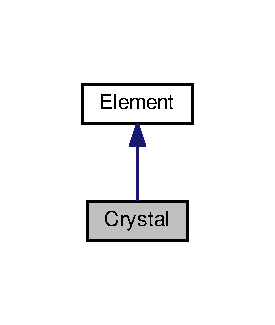
\includegraphics[width=132pt]{classCrystal__inherit__graph}
\end{center}
\end{figure}


Collaboration diagram for Crystal\+:\nopagebreak
\begin{figure}[H]
\begin{center}
\leavevmode
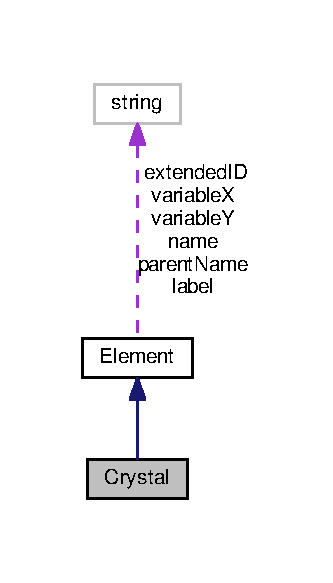
\includegraphics[width=160pt]{classCrystal__coll__graph}
\end{center}
\end{figure}
\subsection*{Public Member Functions}
\begin{DoxyCompactItemize}
\item 
\hypertarget{classCrystal_abb5f724effb4f19e4e3abde2214f0b2f}{{\bfseries Crystal} (const \hyperlink{classCrystal}{Crystal} \&obj)}\label{classCrystal_abb5f724effb4f19e4e3abde2214f0b2f}

\item 
\hypertarget{classCrystal_af70f2647bde3546e79eedfd89710aaac}{\hyperlink{classMppc}{Mppc} $\ast$ {\bfseries Get\+Mppc} ()}\label{classCrystal_af70f2647bde3546e79eedfd89710aaac}

\item 
\hypertarget{classCrystal_a545ad3e5b0aa7181e2c8141483b2ec8e}{T\+H1\+F $\ast$ {\bfseries Get\+Spectrum} ()}\label{classCrystal_a545ad3e5b0aa7181e2c8141483b2ec8e}

\item 
\hypertarget{classCrystal_a302a058bd2f358532b5e5dedb4ef5af1}{T\+H1\+F $\ast$ {\bfseries Get\+Highlighted\+Spectrum} ()}\label{classCrystal_a302a058bd2f358532b5e5dedb4ef5af1}

\item 
\hypertarget{classCrystal_a1662dbae8a3b5d86e010f23ec0023b6b}{T\+H1\+F $\ast$ {\bfseries Get\+Histo\+W} ()}\label{classCrystal_a1662dbae8a3b5d86e010f23ec0023b6b}

\item 
\hypertarget{classCrystal_a00cb7461f242ace491e9be55e7a496e3}{T\+F1 $\ast$ {\bfseries Get\+Fit} ()}\label{classCrystal_a00cb7461f242ace491e9be55e7a496e3}

\item 
\hypertarget{classCrystal_adfc9e1c99c109c6b1656c1c160e1a5dd}{T\+F1 $\ast$ {\bfseries Get\+Sim\+Fit} ()}\label{classCrystal_adfc9e1c99c109c6b1656c1c160e1a5dd}

\item 
\hypertarget{classCrystal_a4d97a11a2bc42b235b336a6c305b9142}{T\+F1 $\ast$ {\bfseries Get\+Histo\+Wfit} ()}\label{classCrystal_a4d97a11a2bc42b235b336a6c305b9142}

\item 
\hypertarget{classCrystal_a290199b0343a255672fc281379a41af7}{double {\bfseries Get\+Wfwhm} ()}\label{classCrystal_a290199b0343a255672fc281379a41af7}

\item 
\hypertarget{classCrystal_adf1de11d276a43661582875060d04042}{double {\bfseries Get\+Wrms} ()}\label{classCrystal_adf1de11d276a43661582875060d04042}

\item 
\hypertarget{classCrystal_a2421f68bf5e18225b32233736bf0e941}{double {\bfseries Get\+Wwidth20perc} ()}\label{classCrystal_a2421f68bf5e18225b32233736bf0e941}

\item 
\hypertarget{classCrystal_a321e8e8aee60ca58a2d7e7ff6f923bdd}{T\+Cut {\bfseries Get\+Crystal\+Cut} ()}\label{classCrystal_a321e8e8aee60ca58a2d7e7ff6f923bdd}

\item 
\hypertarget{classCrystal_a2115d38df8c47c85b7e10ecc35c47b2f}{T\+Ellipse $\ast$ {\bfseries Get\+Graphical\+Cut} ()}\label{classCrystal_a2115d38df8c47c85b7e10ecc35c47b2f}

\item 
\hypertarget{classCrystal_a522e1a3d66cdc40c0d9997b5d1e12541}{float {\bfseries Get\+Photopeak\+Position} ()}\label{classCrystal_a522e1a3d66cdc40c0d9997b5d1e12541}

\item 
\hypertarget{classCrystal_ad569aa2fffeb3e6c2372e8911034e62b}{float {\bfseries Get\+Photopeak\+Sigma} ()}\label{classCrystal_ad569aa2fffeb3e6c2372e8911034e62b}

\item 
\hypertarget{classCrystal_a524f528dd614f83f34a9fb812ea8d736}{float {\bfseries Get\+Photopeak\+Energy\+Resolution} ()}\label{classCrystal_a524f528dd614f83f34a9fb812ea8d736}

\item 
\hypertarget{classCrystal_a35c22232aa809cff0880014868fca953}{bool {\bfseries Crystal\+Is\+On} ()}\label{classCrystal_a35c22232aa809cff0880014868fca953}

\item 
\hypertarget{classCrystal_a9c53022d870dbee0eae995fd96d4d091}{T\+H2\+F $\ast$ {\bfseries Get\+Versus\+Time} ()}\label{classCrystal_a9c53022d870dbee0eae995fd96d4d091}

\item 
\hypertarget{classCrystal_a9134db27f849c3aaedc8e23168dd3d6d}{T\+H2\+F $\ast$ {\bfseries Get\+Sim\+D\+O\+Iplot} ()}\label{classCrystal_a9134db27f849c3aaedc8e23168dd3d6d}

\item 
\hypertarget{classCrystal_a3b46dc782bf50572aac24838d800db5e}{T\+Graph $\ast$ {\bfseries Get\+Sim\+Graph} ()}\label{classCrystal_a3b46dc782bf50572aac24838d800db5e}

\item 
\hypertarget{classCrystal_a48ff2699084705a04f1150c11ab7b401}{double {\bfseries Get\+U} ()}\label{classCrystal_a48ff2699084705a04f1150c11ab7b401}

\item 
\hypertarget{classCrystal_aab99e249407947b60dc54003f2b3323c}{double {\bfseries Get\+V} ()}\label{classCrystal_aab99e249407947b60dc54003f2b3323c}

\item 
\hypertarget{classCrystal_a983a0fcefdc19de4cc6de0b1c04c7f6c}{double {\bfseries Get\+W\+U} ()}\label{classCrystal_a983a0fcefdc19de4cc6de0b1c04c7f6c}

\item 
\hypertarget{classCrystal_a31b8c18bf9feb2a3cf785d3fa35d9b15}{double {\bfseries Get\+W\+V} ()}\label{classCrystal_a31b8c18bf9feb2a3cf785d3fa35d9b15}

\item 
\hypertarget{classCrystal_af73793ea59c22697866867896302d93e}{double {\bfseries Get\+T} ()}\label{classCrystal_af73793ea59c22697866867896302d93e}

\item 
\hypertarget{classCrystal_a8ad8c5364288e3f2abff5ad86ae3eca0}{void {\bfseries Set\+Mppc} (\hyperlink{classMppc}{Mppc} $\ast$amppc)}\label{classCrystal_a8ad8c5364288e3f2abff5ad86ae3eca0}

\item 
\hypertarget{classCrystal_a7ef968f68279b0010ad3abba2e5c5ed1}{void {\bfseries Set\+Spectrum} (T\+H1\+F a\+Histo)}\label{classCrystal_a7ef968f68279b0010ad3abba2e5c5ed1}

\item 
\hypertarget{classCrystal_ab746643d954d1eee7c0be0c0dd0ebd6f}{void {\bfseries Set\+Highlighted\+Spectrum} (T\+H1\+F a\+Histo)}\label{classCrystal_ab746643d954d1eee7c0be0c0dd0ebd6f}

\item 
\hypertarget{classCrystal_ad46ce2e741ee1a485780a3073a6365cf}{void {\bfseries Set\+Histo\+W} (T\+H1\+F a\+Histo)}\label{classCrystal_ad46ce2e741ee1a485780a3073a6365cf}

\item 
\hypertarget{classCrystal_aac912ce5dbdd63d795287db82572e993}{void {\bfseries Set\+Fit} (T\+F1 a\+Fit)}\label{classCrystal_aac912ce5dbdd63d795287db82572e993}

\item 
\hypertarget{classCrystal_aa612c1a9eae1a1f22d79a65d5e6c682d}{void {\bfseries Set\+Histo\+Wfwhm} (double a)}\label{classCrystal_aa612c1a9eae1a1f22d79a65d5e6c682d}

\item 
\hypertarget{classCrystal_a868d1e76014ffd4b09e545211d9c5035}{void {\bfseries Set\+Histo\+Wrms} (double a)}\label{classCrystal_a868d1e76014ffd4b09e545211d9c5035}

\item 
\hypertarget{classCrystal_a12584eddc3ccaad6016281a856af663c}{void {\bfseries Set\+Histo\+Wwidth20perc} (double a)}\label{classCrystal_a12584eddc3ccaad6016281a856af663c}

\item 
\hypertarget{classCrystal_a1f1174ca63c2ce00334ef574b6bebcde}{void {\bfseries Set\+Histo\+Wfit} (T\+F1 a\+Fit)}\label{classCrystal_a1f1174ca63c2ce00334ef574b6bebcde}

\item 
\hypertarget{classCrystal_aedb6cd3684777ec64f2228674cd11ebb}{void {\bfseries Set\+Ellipses} (std\+::string var\+X, std\+::string var\+Y)}\label{classCrystal_aedb6cd3684777ec64f2228674cd11ebb}

\item 
\hypertarget{classCrystal_ad189d917526fc61f21d3b8565bd37fcb}{void {\bfseries Set\+Crystal\+On} (bool abool)}\label{classCrystal_ad189d917526fc61f21d3b8565bd37fcb}

\item 
\hypertarget{classCrystal_aa0c666d8f9ebc01e4a923a897894cf47}{void {\bfseries Set\+Crystal\+Data} (double au, double av, double awu, double awv, double at)}\label{classCrystal_aa0c666d8f9ebc01e4a923a897894cf47}

\item 
\hypertarget{classCrystal_a37815937e4978031c25f0036ea48fba9}{void {\bfseries Set\+Graphical\+Cut} (T\+Ellipse a\+Ellipse)}\label{classCrystal_a37815937e4978031c25f0036ea48fba9}

\item 
\hypertarget{classCrystal_a995cc2d54db8b9e584d5d8675d6cd80d}{void {\bfseries Set\+Photopeak} (float a, float b)}\label{classCrystal_a995cc2d54db8b9e584d5d8675d6cd80d}

\item 
\hypertarget{classCrystal_a6b9b3e253859a88d02122d61d0bb6dda}{void {\bfseries Set\+Versus\+Time} (T\+H2\+F a\+Histo)}\label{classCrystal_a6b9b3e253859a88d02122d61d0bb6dda}

\item 
\hypertarget{classCrystal_a5d364fe8e20a485906fa459f22bc4c0d}{void {\bfseries Set\+Sim\+D\+O\+Iplot} (T\+H2\+F a\+Histo)}\label{classCrystal_a5d364fe8e20a485906fa459f22bc4c0d}

\item 
\hypertarget{classCrystal_a7478983365206faec3b17ce6bf602505}{void {\bfseries Set\+Sim\+Graph} (T\+Graph a\+Graph)}\label{classCrystal_a7478983365206faec3b17ce6bf602505}

\item 
\hypertarget{classCrystal_ab93ab8100f52f7bbb1eae56c78f8ca48}{void {\bfseries Set\+Sim\+Fit} (T\+F1 a\+Fit)}\label{classCrystal_ab93ab8100f52f7bbb1eae56c78f8ca48}

\item 
\hypertarget{classCrystal_a9b84060cc87f2940c6860cd906a3d49d}{void {\bfseries Analyze} ()}\label{classCrystal_a9b84060cc87f2940c6860cd906a3d49d}

\item 
\hypertarget{classCrystal_a3a63627bb261a091eb4f166f455ce268}{void {\bfseries Print\+Global} ()}\label{classCrystal_a3a63627bb261a091eb4f166f455ce268}

\item 
void \hyperlink{classCrystal_a12cf58149ed3037247f27a924c70d411}{Print\+Specific} ()
\begin{DoxyCompactList}\small\item\em prints specific info of this element. polimorphic implementation in the specific class of each elements \end{DoxyCompactList}\end{DoxyCompactItemize}
\subsection*{Additional Inherited Members}


\subsection{Member Function Documentation}
\hypertarget{classCrystal_a12cf58149ed3037247f27a924c70d411}{\index{Crystal@{Crystal}!Print\+Specific@{Print\+Specific}}
\index{Print\+Specific@{Print\+Specific}!Crystal@{Crystal}}
\subsubsection[{Print\+Specific}]{\setlength{\rightskip}{0pt plus 5cm}void Crystal\+::\+Print\+Specific (
\begin{DoxyParamCaption}
{}
\end{DoxyParamCaption}
)\hspace{0.3cm}{\ttfamily [virtual]}}}\label{classCrystal_a12cf58149ed3037247f27a924c70d411}


prints specific info of this element. polimorphic implementation in the specific class of each elements 

Prints \hyperlink{classElement}{Element} info to terminal Variables printed here are specific to this type of element

Reimplemented from \hyperlink{classElement_adef0eb8aa2179a099c38d96217c237c0}{Element}.



The documentation for this class was generated from the following files\+:\begin{DoxyCompactItemize}
\item 
include/Crystal.\+h\item 
src/Crystal.\+cc\end{DoxyCompactItemize}

\hypertarget{classElement}{\section{Element Class Reference}
\label{classElement}\index{Element@{Element}}
}


Inheritance diagram for Element\+:
\nopagebreak
\begin{figure}[H]
\begin{center}
\leavevmode
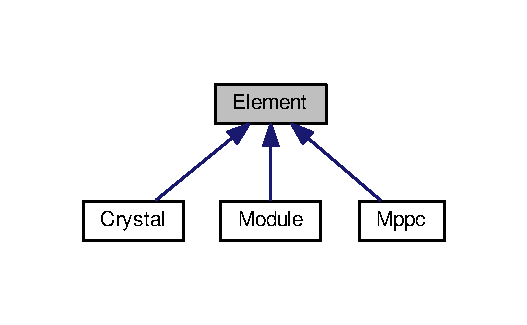
\includegraphics[width=253pt]{classElement__inherit__graph}
\end{center}
\end{figure}


Collaboration diagram for Element\+:
\nopagebreak
\begin{figure}[H]
\begin{center}
\leavevmode
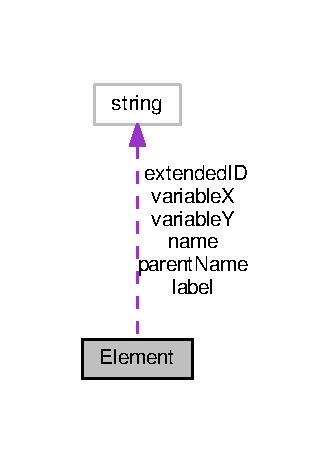
\includegraphics[width=160pt]{classElement__coll__graph}
\end{center}
\end{figure}
\subsection*{Public Member Functions}
\begin{DoxyCompactItemize}
\item 
\hypertarget{classElement_a35c96bb94fc3c42ebb4eab1c51ce2a63}{{\bfseries Element} (const \hyperlink{classElement}{Element} \&obj)}\label{classElement_a35c96bb94fc3c42ebb4eab1c51ce2a63}

\item 
\hypertarget{classElement_aa38eb6cc012786635a632f11ec0c3c41}{std\+::string {\bfseries Get\+Name} ()}\label{classElement_aa38eb6cc012786635a632f11ec0c3c41}

\item 
\hypertarget{classElement_a12f6f5b01cd73e62382f319dbd71129b}{std\+::string {\bfseries Get\+Label} ()}\label{classElement_a12f6f5b01cd73e62382f319dbd71129b}

\item 
\hypertarget{classElement_a01c2709f33fe0773cad6089e8fc7261b}{int {\bfseries Get\+I\+D} ()}\label{classElement_a01c2709f33fe0773cad6089e8fc7261b}

\item 
\hypertarget{classElement_afedae45e6b3dd9f9a66a68a6e2acb937}{std\+::string {\bfseries Get\+Extended\+I\+D} ()}\label{classElement_afedae45e6b3dd9f9a66a68a6e2acb937}

\item 
\hypertarget{classElement_aa192e6c35a460ea561021f3b37c6700a}{int {\bfseries Get\+I} ()}\label{classElement_aa192e6c35a460ea561021f3b37c6700a}

\item 
\hypertarget{classElement_afb05febdece810f4b83541624fe530ee}{int {\bfseries Get\+J} ()}\label{classElement_afb05febdece810f4b83541624fe530ee}

\item 
\hypertarget{classElement_a0642f0da63632170f9fa9df021c977f1}{float {\bfseries Get\+X} ()}\label{classElement_a0642f0da63632170f9fa9df021c977f1}

\item 
\hypertarget{classElement_a4c4f314d040db786a716ed916a42ebd7}{float {\bfseries Get\+Y} ()}\label{classElement_a4c4f314d040db786a716ed916a42ebd7}

\item 
\hypertarget{classElement_af03625767fde8b12a09add84108c3f2d}{float {\bfseries Get\+Z} ()}\label{classElement_af03625767fde8b12a09add84108c3f2d}

\item 
\hypertarget{classElement_ad02bc3fa1779c70ae5f71da8569e4a25}{float {\bfseries Get\+Dimension\+X} ()}\label{classElement_ad02bc3fa1779c70ae5f71da8569e4a25}

\item 
\hypertarget{classElement_ac09017b6bb0145f254e6196350e4a2f3}{float {\bfseries Get\+Dimension\+Y} ()}\label{classElement_ac09017b6bb0145f254e6196350e4a2f3}

\item 
\hypertarget{classElement_abd9535fcf6b5918a090c68f13088f483}{float {\bfseries Get\+Dimension\+Z} ()}\label{classElement_abd9535fcf6b5918a090c68f13088f483}

\item 
\hypertarget{classElement_abec5fea86c8be1bfc8e797a5f72152c4}{int {\bfseries Get\+Children\+I} ()}\label{classElement_abec5fea86c8be1bfc8e797a5f72152c4}

\item 
\hypertarget{classElement_a11b2a4ce751161ef1752fd3a39493268}{int {\bfseries Get\+Children\+J} ()}\label{classElement_a11b2a4ce751161ef1752fd3a39493268}

\item 
\hypertarget{classElement_a8da798fc7a492f6d68c32e72e3764906}{std\+::string {\bfseries Get\+Parent\+Name} ()}\label{classElement_a8da798fc7a492f6d68c32e72e3764906}

\item 
\hypertarget{classElement_ab58130947efb1126d566e5074fbe2a98}{T\+H2\+F $\ast$ {\bfseries Get\+Flood\+Map2\+D} ()}\label{classElement_ab58130947efb1126d566e5074fbe2a98}

\item 
\hypertarget{classElement_aea2af6bb32440632f398d12e6fb6db9d}{T\+H2\+F $\ast$ {\bfseries Get\+A\+D\+Cversus\+W} ()}\label{classElement_aea2af6bb32440632f398d12e6fb6db9d}

\item 
\hypertarget{classElement_a97ef42c709b407a4c17289e7c91218dd}{T\+H2\+F $\ast$ {\bfseries Get\+Flood\+Map2\+D\+Separated} ()}\label{classElement_a97ef42c709b407a4c17289e7c91218dd}

\item 
\hypertarget{classElement_a92e1e05aedd6727139a11dc942a3b129}{T\+H2\+F $\ast$ {\bfseries Get\+Spherical\+Map} ()}\label{classElement_a92e1e05aedd6727139a11dc942a3b129}

\item 
\hypertarget{classElement_a2c335eb77b8583ddd2c24953f92da87a}{T\+H2\+F $\ast$ {\bfseries Get\+Cylindrical\+X\+Map} ()}\label{classElement_a2c335eb77b8583ddd2c24953f92da87a}

\item 
\hypertarget{classElement_aa4a66652df9933e017d278a21faef72c}{T\+H2\+F $\ast$ {\bfseries Get\+Cylindrical\+Y\+Map} ()}\label{classElement_aa4a66652df9933e017d278a21faef72c}

\item 
\hypertarget{classElement_a57fcfb4d3c56183ec07432416d656be4}{T\+H2\+F $\ast$ {\bfseries Get\+Lateral\+Map} ()}\label{classElement_a57fcfb4d3c56183ec07432416d656be4}

\item 
\hypertarget{classElement_a8097c9a1f83cd9addb5cec2a16c03f3a}{T\+H2\+F $\ast$ {\bfseries Get\+Corner\+Map} ()}\label{classElement_a8097c9a1f83cd9addb5cec2a16c03f3a}

\item 
\hypertarget{classElement_aa3e4f19eca1295d8e1850184e6c7be04}{T\+H2\+F $\ast$ {\bfseries Get\+Central\+Map} ()}\label{classElement_aa3e4f19eca1295d8e1850184e6c7be04}

\item 
\hypertarget{classElement_a997c6d58ec6c513b4e5a072a16a5f902}{T\+H3\+F $\ast$ {\bfseries Get\+Flood\+Map3\+D} ()}\label{classElement_a997c6d58ec6c513b4e5a072a16a5f902}

\item 
\hypertarget{classElement_a1f70d930511a1c18022e26fa216ed368}{std\+::string {\bfseries Get\+Xvariable} ()}\label{classElement_a1f70d930511a1c18022e26fa216ed368}

\item 
\hypertarget{classElement_aa165d8d22f634aa55df220ddac6cd6b6}{std\+::string {\bfseries Get\+Yvariable} ()}\label{classElement_aa165d8d22f634aa55df220ddac6cd6b6}

\item 
\hypertarget{classElement_a9fb68ca0150cdac10c437ea9e1ac6e35}{void {\bfseries Set\+Name} (std\+::string aname)}\label{classElement_a9fb68ca0150cdac10c437ea9e1ac6e35}

\item 
\hypertarget{classElement_a2f4977024fc457839ac3d7213c1a161e}{void {\bfseries Set\+Label} (std\+::string aname)}\label{classElement_a2f4977024fc457839ac3d7213c1a161e}

\item 
\hypertarget{classElement_adeed13224a6b76fe25692693116190da}{void {\bfseries Set\+I\+D} (int pid)}\label{classElement_adeed13224a6b76fe25692693116190da}

\item 
\hypertarget{classElement_add696c642cf2c66a0f533e3547d1aa6f}{void {\bfseries Set\+Extended\+I\+D} (std\+::string pid)}\label{classElement_add696c642cf2c66a0f533e3547d1aa6f}

\item 
\hypertarget{classElement_a326a0b4c9e0c9ffabd143587f8a41b3b}{void {\bfseries Set\+I} (int pi)}\label{classElement_a326a0b4c9e0c9ffabd143587f8a41b3b}

\item 
\hypertarget{classElement_ab7c7f57f6089a3a9e2b1123627a8d7bc}{void {\bfseries Set\+J} (int pj)}\label{classElement_ab7c7f57f6089a3a9e2b1123627a8d7bc}

\item 
\hypertarget{classElement_a39ff32a2cc85f79498d9346df5e8d70c}{void {\bfseries Set\+Position} (float px, float py, float pz)}\label{classElement_a39ff32a2cc85f79498d9346df5e8d70c}

\item 
\hypertarget{classElement_a755ef6c37fe68010d51615218b3c2e52}{void {\bfseries Set\+Dimension} (float px, float py, float pz)}\label{classElement_a755ef6c37fe68010d51615218b3c2e52}

\item 
\hypertarget{classElement_a907a8df082b331f560d4be0ea5e97576}{void {\bfseries Set\+Children\+I} (int pi)}\label{classElement_a907a8df082b331f560d4be0ea5e97576}

\item 
\hypertarget{classElement_a7e75b4ef17047487124c3df65e460b18}{void {\bfseries Set\+Children\+J} (int pj)}\label{classElement_a7e75b4ef17047487124c3df65e460b18}

\item 
\hypertarget{classElement_a35030032beef99b7eb1181022cc55b1a}{void {\bfseries Set\+Parent\+Name} (std\+::string a\+Name)}\label{classElement_a35030032beef99b7eb1181022cc55b1a}

\item 
\hypertarget{classElement_a8c690d49d503ef39b0d8ae8eb553fb93}{void {\bfseries Set\+Flood\+Map2\+D} (T\+H2\+F a\+Histo)}\label{classElement_a8c690d49d503ef39b0d8ae8eb553fb93}

\item 
\hypertarget{classElement_a52e5e8e7a1f4c0396d3d5c7d7503ba16}{void {\bfseries Set\+A\+D\+Cversus\+W} (T\+H2\+F a\+Histo)}\label{classElement_a52e5e8e7a1f4c0396d3d5c7d7503ba16}

\item 
\hypertarget{classElement_a9744147b64996c8dd2211bc821effc93}{void {\bfseries Set\+Flood\+Map2\+D\+Separated} (T\+H2\+F a\+Histo)}\label{classElement_a9744147b64996c8dd2211bc821effc93}

\item 
\hypertarget{classElement_a407ed6b0127ab9313b95a1489fdf7a42}{void {\bfseries Set\+Spherical\+Map} (T\+H2\+F a\+Histo)}\label{classElement_a407ed6b0127ab9313b95a1489fdf7a42}

\item 
\hypertarget{classElement_abcdb076f522e0e679003d92ea549fe85}{void {\bfseries Set\+Cylindrical\+X\+Map} (T\+H2\+F a\+Histo)}\label{classElement_abcdb076f522e0e679003d92ea549fe85}

\item 
\hypertarget{classElement_a46aabe074a344e8a0a31eff4e9fbfd32}{void {\bfseries Set\+Cylindrical\+Y\+Map} (T\+H2\+F a\+Histo)}\label{classElement_a46aabe074a344e8a0a31eff4e9fbfd32}

\item 
\hypertarget{classElement_a0cba0637b48af6109844ab470084d861}{void {\bfseries Set\+Flood\+Map3\+D} (T\+H3\+F a\+Histo)}\label{classElement_a0cba0637b48af6109844ab470084d861}

\item 
\hypertarget{classElement_a50762fc0cc57a191f09f50049be2ac0e}{void {\bfseries Set\+Lateral\+Map} (T\+H2\+F a\+Histo)}\label{classElement_a50762fc0cc57a191f09f50049be2ac0e}

\item 
\hypertarget{classElement_aabc88cb1a289df02cc74f17a7fc8992e}{void {\bfseries Set\+Corner\+Map} (T\+H2\+F a\+Histo)}\label{classElement_aabc88cb1a289df02cc74f17a7fc8992e}

\item 
\hypertarget{classElement_a207f6ae9fd0afda9c7dd6d6273ffc0ba}{void {\bfseries Set\+Central\+Map} (T\+H2\+F a\+Histo)}\label{classElement_a207f6ae9fd0afda9c7dd6d6273ffc0ba}

\item 
\hypertarget{classElement_acb619fc989012adef1de6f79639f0f77}{void {\bfseries Set\+Xvariable} (std\+::string astring)}\label{classElement_acb619fc989012adef1de6f79639f0f77}

\item 
\hypertarget{classElement_aca1f8fb595b4d35c482bc1ebc7eee4d6}{void {\bfseries Set\+Yvariable} (std\+::string astring)}\label{classElement_aca1f8fb595b4d35c482bc1ebc7eee4d6}

\item 
\hypertarget{classElement_a18af20eae501f4e74e17663f5295e842}{void {\bfseries Add\+Child} (std\+::string a\+Name)}\label{classElement_a18af20eae501f4e74e17663f5295e842}

\item 
\hypertarget{classElement_ab027b4d21940058225371012e3e9ce37}{std\+::vector$<$ std\+::string $>$ {\bfseries Get\+Children} ()}\label{classElement_ab027b4d21940058225371012e3e9ce37}

\item 
\hypertarget{classElement_afcde5aa81a52b90a8bcf903d9b773ebc}{void {\bfseries Print\+Global} ()}\label{classElement_afcde5aa81a52b90a8bcf903d9b773ebc}

\item 
\hypertarget{classElement_adef0eb8aa2179a099c38d96217c237c0}{virtual void {\bfseries Print\+Specific} ()}\label{classElement_adef0eb8aa2179a099c38d96217c237c0}

\item 
\hypertarget{classElement_a623ce34f0347c395e33e79ef43d9b93d}{void {\bfseries Print} ()}\label{classElement_a623ce34f0347c395e33e79ef43d9b93d}

\end{DoxyCompactItemize}
\subsection*{Protected Attributes}
\begin{DoxyCompactItemize}
\item 
\hypertarget{classElement_a159736231f5227e65e36f4a9e5537afd}{std\+::string {\bfseries name}}\label{classElement_a159736231f5227e65e36f4a9e5537afd}

\item 
\hypertarget{classElement_a2e3029a6dec4d74046ce1e4efe72d5f7}{std\+::string {\bfseries label}}\label{classElement_a2e3029a6dec4d74046ce1e4efe72d5f7}

\item 
\hypertarget{classElement_abe6237e9f33c87cca4e24ed5ebc51bfb}{std\+::string {\bfseries parent\+Name}}\label{classElement_abe6237e9f33c87cca4e24ed5ebc51bfb}

\item 
\hypertarget{classElement_ab1248ff46559a0cb27d56568e6e479f5}{std\+::vector$<$ std\+::string $>$ {\bfseries children\+Name}}\label{classElement_ab1248ff46559a0cb27d56568e6e479f5}

\item 
\hypertarget{classElement_aff44a78d101de8f17f4448e0bc65e4a2}{std\+::string {\bfseries extended\+I\+D}}\label{classElement_aff44a78d101de8f17f4448e0bc65e4a2}

\item 
\hypertarget{classElement_ab176775b7d8a64ad8a8cc24e1f0f3d3f}{std\+::string {\bfseries variable\+X}}\label{classElement_ab176775b7d8a64ad8a8cc24e1f0f3d3f}

\item 
\hypertarget{classElement_ad34ac2c8cf07782f878b2ae48f69c4c4}{std\+::string {\bfseries variable\+Y}}\label{classElement_ad34ac2c8cf07782f878b2ae48f69c4c4}

\item 
\hypertarget{classElement_a3bd136c994cd7b24a62cb464f78990ad}{int {\bfseries id}}\label{classElement_a3bd136c994cd7b24a62cb464f78990ad}

\item 
\hypertarget{classElement_ae973e652f252c0d41cf2f251c07fcf30}{int {\bfseries i}}\label{classElement_ae973e652f252c0d41cf2f251c07fcf30}

\item 
\hypertarget{classElement_afc114c80c73d8264637ab15b022a6ad2}{int {\bfseries j}}\label{classElement_afc114c80c73d8264637ab15b022a6ad2}

\item 
\hypertarget{classElement_a32de6866d49c3cd4634f290fde2280d3}{float {\bfseries x}}\label{classElement_a32de6866d49c3cd4634f290fde2280d3}

\item 
\hypertarget{classElement_a39fa54b6d5c56d067748a8e13f0be851}{float {\bfseries y}}\label{classElement_a39fa54b6d5c56d067748a8e13f0be851}

\item 
\hypertarget{classElement_a9673a121290573dd806820bbdf5a5c27}{float {\bfseries z}}\label{classElement_a9673a121290573dd806820bbdf5a5c27}

\item 
\hypertarget{classElement_a596ef7a8bf00c43ec69ab34552e0bcf5}{float {\bfseries dx}}\label{classElement_a596ef7a8bf00c43ec69ab34552e0bcf5}

\item 
\hypertarget{classElement_a8fb86b3d6acc44716d46124fe1ca3910}{float {\bfseries dy}}\label{classElement_a8fb86b3d6acc44716d46124fe1ca3910}

\item 
\hypertarget{classElement_a14e5f51fbe61d3bdbbe4d44c65f03dc5}{float {\bfseries dz}}\label{classElement_a14e5f51fbe61d3bdbbe4d44c65f03dc5}

\item 
\hypertarget{classElement_a37c5bed50bec96560c89fddb9dd10d6a}{int {\bfseries i\+Children}}\label{classElement_a37c5bed50bec96560c89fddb9dd10d6a}

\item 
\hypertarget{classElement_a7347c8c6c06759f8ae2a2cd15543c85b}{int {\bfseries j\+Children}}\label{classElement_a7347c8c6c06759f8ae2a2cd15543c85b}

\item 
\hypertarget{classElement_adb8076cb5e85bbd5b22ff0469fbf120c}{T\+H2\+F {\bfseries Flood\+Map2\+D}}\label{classElement_adb8076cb5e85bbd5b22ff0469fbf120c}

\item 
\hypertarget{classElement_a6e1fe25cbd51761ff59d92bfd380b58e}{T\+H2\+F {\bfseries Flood\+Map2\+D\+Separated}}\label{classElement_a6e1fe25cbd51761ff59d92bfd380b58e}

\item 
\hypertarget{classElement_acbf98095e81976bfad9aa6a0cae62687}{T\+H2\+F {\bfseries Spherical\+Map}}\label{classElement_acbf98095e81976bfad9aa6a0cae62687}

\item 
\hypertarget{classElement_a41a0b90394cc0d4460c47566eeba6739}{T\+H2\+F {\bfseries Cylindrical\+X\+Map}}\label{classElement_a41a0b90394cc0d4460c47566eeba6739}

\item 
\hypertarget{classElement_ac147ebacd2963fb1ef2baed0014e160c}{T\+H2\+F {\bfseries Cylindrical\+Y\+Map}}\label{classElement_ac147ebacd2963fb1ef2baed0014e160c}

\item 
\hypertarget{classElement_a82cfb891b137602dc49bbb18c1039b5c}{T\+H2\+F {\bfseries Lateral\+Map}}\label{classElement_a82cfb891b137602dc49bbb18c1039b5c}

\item 
\hypertarget{classElement_ad01d15c50d4d01716f8d9d03162521f9}{T\+H2\+F {\bfseries Corner\+Map}}\label{classElement_ad01d15c50d4d01716f8d9d03162521f9}

\item 
\hypertarget{classElement_ac25c0eb24baee3f0b3228b6279791d21}{T\+H2\+F {\bfseries Central\+Map}}\label{classElement_ac25c0eb24baee3f0b3228b6279791d21}

\item 
\hypertarget{classElement_a62ed98e003ba00fee131353869cfe314}{T\+H2\+F {\bfseries A\+D\+Cversus\+W}}\label{classElement_a62ed98e003ba00fee131353869cfe314}

\item 
\hypertarget{classElement_a97f8372319c77f20eff4314a6f32c4ad}{T\+H3\+F {\bfseries Flood\+Map3\+D}}\label{classElement_a97f8372319c77f20eff4314a6f32c4ad}

\end{DoxyCompactItemize}


The documentation for this class was generated from the following files\+:\begin{DoxyCompactItemize}
\item 
include/Element.\+h\item 
src/Element.\+cc\end{DoxyCompactItemize}

\hypertarget{structConfigFile_1_1file__not__found}{\section{Config\+File\+:\+:file\+\_\+not\+\_\+found Struct Reference}
\label{structConfigFile_1_1file__not__found}\index{Config\+File\+::file\+\_\+not\+\_\+found@{Config\+File\+::file\+\_\+not\+\_\+found}}
}


Collaboration diagram for Config\+File\+:\+:file\+\_\+not\+\_\+found\+:
\nopagebreak
\begin{figure}[H]
\begin{center}
\leavevmode
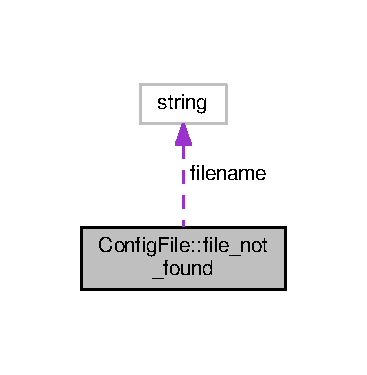
\includegraphics[width=176pt]{structConfigFile_1_1file__not__found__coll__graph}
\end{center}
\end{figure}
\subsection*{Public Member Functions}
\begin{DoxyCompactItemize}
\item 
\hypertarget{structConfigFile_1_1file__not__found_ab0fa2b6e7d1891136f82d4baf124725b}{{\bfseries file\+\_\+not\+\_\+found} (const string \&filename\+\_\+=string())}\label{structConfigFile_1_1file__not__found_ab0fa2b6e7d1891136f82d4baf124725b}

\end{DoxyCompactItemize}
\subsection*{Public Attributes}
\begin{DoxyCompactItemize}
\item 
\hypertarget{structConfigFile_1_1file__not__found_a25e11d11b1a9b0f4ca663b21816c2a9a}{string {\bfseries filename}}\label{structConfigFile_1_1file__not__found_a25e11d11b1a9b0f4ca663b21816c2a9a}

\end{DoxyCompactItemize}


The documentation for this struct was generated from the following file\+:\begin{DoxyCompactItemize}
\item 
include/Config\+File.\+h\end{DoxyCompactItemize}

\hypertarget{classInputFile}{\section{Input\+File Class Reference}
\label{classInputFile}\index{Input\+File@{Input\+File}}
}


Collaboration diagram for Input\+File\+:
\nopagebreak
\begin{figure}[H]
\begin{center}
\leavevmode
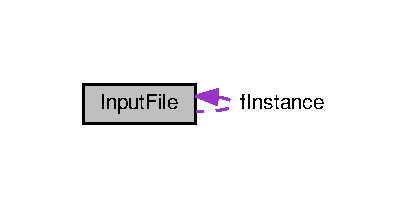
\includegraphics[width=196pt]{classInputFile__coll__graph}
\end{center}
\end{figure}
\subsection*{Public Member Functions}
\begin{DoxyCompactItemize}
\item 
\hypertarget{classInputFile_a1e310e7fc2da2ba81f2b959661625af6}{{\bfseries Input\+File} (int argc, char $\ast$$\ast$argv, \hyperlink{classConfigFile}{Config\+File} \&config)}\label{classInputFile_a1e310e7fc2da2ba81f2b959661625af6}

\item 
\hypertarget{classInputFile_a948e7cc1141e3f3b05fbbf836408a085}{T\+Chain $\ast$ {\bfseries Get\+Chain} () const }\label{classInputFile_a948e7cc1141e3f3b05fbbf836408a085}

\item 
\hypertarget{classInputFile_a2ab271cc4fac7e35b43d97b5901eeac8}{T\+Tree $\ast$ {\bfseries Get\+Tree} () const }\label{classInputFile_a2ab271cc4fac7e35b43d97b5901eeac8}

\item 
\hypertarget{classInputFile_a3dc20eebe07374d6abbc83c39744c464}{void {\bfseries Create\+Tree} ()}\label{classInputFile_a3dc20eebe07374d6abbc83c39744c464}

\item 
\hypertarget{classInputFile_ae4004a365b09e90a562732bc761e1cb5}{void {\bfseries Fill\+Elements} (\hyperlink{classModule}{Module} $\ast$$\ast$$\ast$module, \hyperlink{classMppc}{Mppc} $\ast$$\ast$$\ast$mppc, \hyperlink{classCrystal}{Crystal} $\ast$$\ast$$\ast$crystal)}\label{classInputFile_ae4004a365b09e90a562732bc761e1cb5}

\end{DoxyCompactItemize}
\subsection*{Static Public Member Functions}
\begin{DoxyCompactItemize}
\item 
\hypertarget{classInputFile_acd483270b7e4223f2a655c7badb5736a}{static \hyperlink{classInputFile}{Input\+File} $\ast$ {\bfseries Instance} ()}\label{classInputFile_acd483270b7e4223f2a655c7badb5736a}

\end{DoxyCompactItemize}
\subsection*{Static Public Attributes}
\begin{DoxyCompactItemize}
\item 
\hypertarget{classInputFile_ae5318f9a5f1d3d68e3d3f67388c6090f}{static \hyperlink{classInputFile}{Input\+File} $\ast$ {\bfseries f\+Instance}}\label{classInputFile_ae5318f9a5f1d3d68e3d3f67388c6090f}

\end{DoxyCompactItemize}


The documentation for this class was generated from the following files\+:\begin{DoxyCompactItemize}
\item 
include/Input\+File.\+h\item 
src/Input\+File.\+cc\end{DoxyCompactItemize}

\hypertarget{structConfigFile_1_1key__not__found}{\section{Config\+File\+:\+:key\+\_\+not\+\_\+found Struct Reference}
\label{structConfigFile_1_1key__not__found}\index{Config\+File\+::key\+\_\+not\+\_\+found@{Config\+File\+::key\+\_\+not\+\_\+found}}
}


Collaboration diagram for Config\+File\+:\+:key\+\_\+not\+\_\+found\+:\nopagebreak
\begin{figure}[H]
\begin{center}
\leavevmode
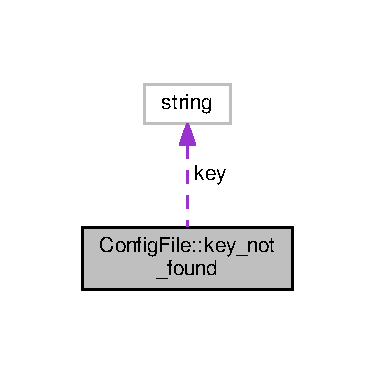
\includegraphics[width=180pt]{structConfigFile_1_1key__not__found__coll__graph}
\end{center}
\end{figure}
\subsection*{Public Member Functions}
\begin{DoxyCompactItemize}
\item 
\hypertarget{structConfigFile_1_1key__not__found_aedacf2df70a4aa179448706b4862d768}{{\bfseries key\+\_\+not\+\_\+found} (const string \&key\+\_\+=string())}\label{structConfigFile_1_1key__not__found_aedacf2df70a4aa179448706b4862d768}

\end{DoxyCompactItemize}
\subsection*{Public Attributes}
\begin{DoxyCompactItemize}
\item 
\hypertarget{structConfigFile_1_1key__not__found_a2872cbeb5ab860f357b3a58dd867b90b}{string {\bfseries key}}\label{structConfigFile_1_1key__not__found_a2872cbeb5ab860f357b3a58dd867b90b}

\end{DoxyCompactItemize}


The documentation for this struct was generated from the following file\+:\begin{DoxyCompactItemize}
\item 
include/Config\+File.\+h\end{DoxyCompactItemize}

\hypertarget{classModule}{\section{Module Class Reference}
\label{classModule}\index{Module@{Module}}
}


Inheritance diagram for Module\+:\nopagebreak
\begin{figure}[H]
\begin{center}
\leavevmode
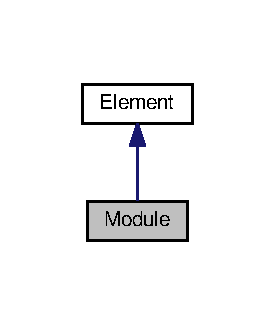
\includegraphics[width=132pt]{classModule__inherit__graph}
\end{center}
\end{figure}


Collaboration diagram for Module\+:\nopagebreak
\begin{figure}[H]
\begin{center}
\leavevmode
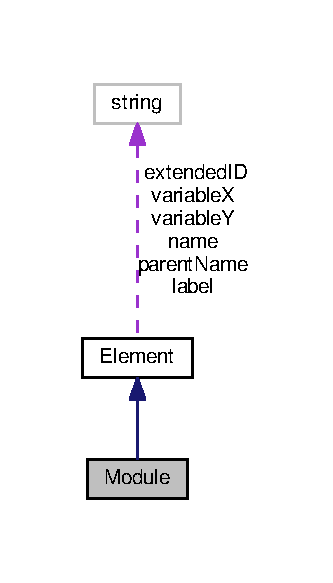
\includegraphics[width=160pt]{classModule__coll__graph}
\end{center}
\end{figure}
\subsection*{Public Member Functions}
\begin{DoxyCompactItemize}
\item 
\hypertarget{classModule_a0b67e6a01ed05b519f53a071f02f0fed}{{\bfseries Module} (const \hyperlink{classModule}{Module} \&obj)}\label{classModule_a0b67e6a01ed05b519f53a071f02f0fed}

\item 
\hypertarget{classModule_a1cbfcfa25abd8fd7cd1054ef71e8e115}{void {\bfseries Set\+Mppc} (\hyperlink{classMppc}{Mppc} $\ast$p\+Mppc)}\label{classModule_a1cbfcfa25abd8fd7cd1054ef71e8e115}

\item 
\hypertarget{classModule_a274245fd0e6f56c534748d7f6186a08f}{int {\bfseries Get\+Mppcs\+Number} ()}\label{classModule_a274245fd0e6f56c534748d7f6186a08f}

\item 
\hypertarget{classModule_ac898a09f44040eccedbf89bde29e4d2b}{\hyperlink{classMppc}{Mppc} $\ast$ {\bfseries Get\+Mppc} (int pi, int pj)}\label{classModule_ac898a09f44040eccedbf89bde29e4d2b}

\item 
\hypertarget{classModule_a16ed7ea902b71f00be9c198da93b5d54}{void {\bfseries Print\+Global} ()}\label{classModule_a16ed7ea902b71f00be9c198da93b5d54}

\item 
void \hyperlink{classModule_af48d2b96b740b2bce1c4435f089ed515}{Print\+Specific} ()
\begin{DoxyCompactList}\small\item\em prints specific info of this element. polimorphic implementation in the specific class of each elements \end{DoxyCompactList}\end{DoxyCompactItemize}
\subsection*{Additional Inherited Members}


\subsection{Member Function Documentation}
\hypertarget{classModule_af48d2b96b740b2bce1c4435f089ed515}{\index{Module@{Module}!Print\+Specific@{Print\+Specific}}
\index{Print\+Specific@{Print\+Specific}!Module@{Module}}
\subsubsection[{Print\+Specific}]{\setlength{\rightskip}{0pt plus 5cm}void Module\+::\+Print\+Specific (
\begin{DoxyParamCaption}
{}
\end{DoxyParamCaption}
)\hspace{0.3cm}{\ttfamily [virtual]}}}\label{classModule_af48d2b96b740b2bce1c4435f089ed515}


prints specific info of this element. polimorphic implementation in the specific class of each elements 

Prints \hyperlink{classElement}{Element} info to terminal Variables printed here are specific to this type of element

Reimplemented from \hyperlink{classElement_adef0eb8aa2179a099c38d96217c237c0}{Element}.



The documentation for this class was generated from the following files\+:\begin{DoxyCompactItemize}
\item 
include/Module.\+h\item 
src/Module.\+cc\end{DoxyCompactItemize}

\hypertarget{classMppc}{\section{Mppc Class Reference}
\label{classMppc}\index{Mppc@{Mppc}}
}


Inheritance diagram for Mppc\+:
\nopagebreak
\begin{figure}[H]
\begin{center}
\leavevmode
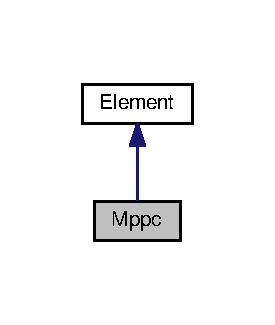
\includegraphics[width=132pt]{classMppc__inherit__graph}
\end{center}
\end{figure}


Collaboration diagram for Mppc\+:
\nopagebreak
\begin{figure}[H]
\begin{center}
\leavevmode
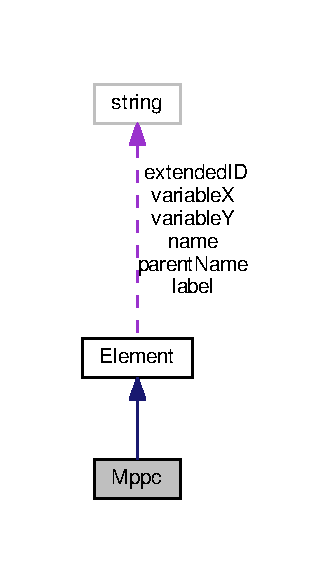
\includegraphics[width=160pt]{classMppc__coll__graph}
\end{center}
\end{figure}
\subsection*{Public Member Functions}
\begin{DoxyCompactItemize}
\item 
\hypertarget{classMppc_adfebdf8d81f516f4f7a52bacd3441a61}{{\bfseries Mppc} (const \hyperlink{classMppc}{Mppc} \&obj)}\label{classMppc_adfebdf8d81f516f4f7a52bacd3441a61}

\item 
\hypertarget{classMppc_a555b0e14d402d9bbab731d861b7402b4}{void {\bfseries Set\+Module} (\hyperlink{classModule}{Module} $\ast$amodule)}\label{classMppc_a555b0e14d402d9bbab731d861b7402b4}

\item 
\hypertarget{classMppc_a4c15acca1a26848d60658676f0b4c341}{\hyperlink{classModule}{Module} $\ast$ {\bfseries Get\+Module} ()}\label{classMppc_a4c15acca1a26848d60658676f0b4c341}

\item 
\hypertarget{classMppc_aa6173b1e462ad6e03263b7e318a34b53}{void {\bfseries Set\+Digitizer\+Channel} (int num)}\label{classMppc_aa6173b1e462ad6e03263b7e318a34b53}

\item 
\hypertarget{classMppc_ae28c74edaf329a243ae48361eb655c6b}{int {\bfseries Get\+Digitizer\+Channel} ()}\label{classMppc_ae28c74edaf329a243ae48361eb655c6b}

\item 
\hypertarget{classMppc_a2ef23bc91e21bf79f15cf635934cec04}{void {\bfseries Set\+Canvas\+Position} (int num)}\label{classMppc_a2ef23bc91e21bf79f15cf635934cec04}

\item 
\hypertarget{classMppc_a16bb7273a7d58849a812c923ac26be72}{int {\bfseries Get\+Canvas\+Position} ()}\label{classMppc_a16bb7273a7d58849a812c923ac26be72}

\item 
\hypertarget{classMppc_aa7cc8b6a7e131a7eb9e97b6b3f0a5425}{void {\bfseries Set\+Crystal} (\hyperlink{classCrystal}{Crystal} $\ast$p\+Crystal)}\label{classMppc_aa7cc8b6a7e131a7eb9e97b6b3f0a5425}

\item 
\hypertarget{classMppc_a956d11c9e8edd85c3d1d3f6793488571}{int {\bfseries Get\+Crystals\+Number} ()}\label{classMppc_a956d11c9e8edd85c3d1d3f6793488571}

\item 
\hypertarget{classMppc_a2c36ef1ffbafb2f475d6968b7d7edc6f}{\hyperlink{classCrystal}{Crystal} $\ast$ {\bfseries Get\+Crystal} (int pi, int pj)}\label{classMppc_a2c36ef1ffbafb2f475d6968b7d7edc6f}

\item 
\hypertarget{classMppc_aeeed71effe5210a9fe5ea4086dd99c6d}{T\+H1\+F $\ast$ {\bfseries Get\+Raw\+Spectrum} ()}\label{classMppc_aeeed71effe5210a9fe5ea4086dd99c6d}

\item 
\hypertarget{classMppc_a05ae0e638488d7ca7a2a7e8c223c7672}{void {\bfseries Set\+Raw\+Spectrum} (T\+H1\+F a\+Histo)}\label{classMppc_a05ae0e638488d7ca7a2a7e8c223c7672}

\item 
\hypertarget{classMppc_a829b437d3969c69f64b36f5ef5622017}{T\+H1\+F $\ast$ {\bfseries Get\+Trigger\+Spectrum} ()}\label{classMppc_a829b437d3969c69f64b36f5ef5622017}

\item 
\hypertarget{classMppc_acf55cba4b46c96dc4d80a9bbf565fe5b}{void {\bfseries Set\+Trigger\+Spectrum} (T\+H1\+F a\+Histo)}\label{classMppc_acf55cba4b46c96dc4d80a9bbf565fe5b}

\item 
\hypertarget{classMppc_a8796833b3eed967559c06608fa9c4bd2}{void {\bfseries Set\+Is\+On\+For\+Doi} (bool abool)}\label{classMppc_a8796833b3eed967559c06608fa9c4bd2}

\item 
\hypertarget{classMppc_a9cfa11f6573aba4e60b46486a4432825}{bool {\bfseries Get\+Is\+On\+For\+Doi} ()}\label{classMppc_a9cfa11f6573aba4e60b46486a4432825}

\item 
\hypertarget{classMppc_ac328d7b2056d789d6fc5d2d7fad40a46}{int {\bfseries Find2\+Dpeaks} ()}\label{classMppc_ac328d7b2056d789d6fc5d2d7fad40a46}

\item 
\hypertarget{classMppc_ac9ee63497a9c7d0fce0c8a03f6f337dd}{void {\bfseries Print\+Global} ()}\label{classMppc_ac9ee63497a9c7d0fce0c8a03f6f337dd}

\item 
\hypertarget{classMppc_aab23e14995583c428c4cce1879936601}{void {\bfseries Print\+Specific} ()}\label{classMppc_aab23e14995583c428c4cce1879936601}

\end{DoxyCompactItemize}
\subsection*{Additional Inherited Members}


The documentation for this class was generated from the following files\+:\begin{DoxyCompactItemize}
\item 
include/Mppc.\+h\item 
src/Mppc.\+cc\end{DoxyCompactItemize}

\hypertarget{structPoint}{\section{Point Struct Reference}
\label{structPoint}\index{Point@{Point}}
}
\subsection*{Public Attributes}
\begin{DoxyCompactItemize}
\item 
\hypertarget{structPoint_a05dfe2dfbde813ad234b514f30e662f1}{float {\bfseries x}}\label{structPoint_a05dfe2dfbde813ad234b514f30e662f1}

\item 
\hypertarget{structPoint_a6101960c8d2d4e8ea1d32c9234bbeb8d}{float {\bfseries y}}\label{structPoint_a6101960c8d2d4e8ea1d32c9234bbeb8d}

\item 
\hypertarget{structPoint_a9a666531e0e99adff132be93d2407d0c}{float {\bfseries z}}\label{structPoint_a9a666531e0e99adff132be93d2407d0c}

\end{DoxyCompactItemize}


The documentation for this struct was generated from the following file\+:\begin{DoxyCompactItemize}
\item 
src/Input\+File.\+cc\end{DoxyCompactItemize}

\hypertarget{structConfigFile_1_1split__t}{\section{Config\+File\+:\+:split\+\_\+t Struct Reference}
\label{structConfigFile_1_1split__t}\index{Config\+File\+::split\+\_\+t@{Config\+File\+::split\+\_\+t}}
}
\subsection*{Public Types}
\begin{DoxyCompactItemize}
\item 
\hypertarget{structConfigFile_1_1split__t_a1e55e44eb3c3693f1a2008115b5aa1e6}{enum {\bfseries empties\+\_\+t} \{ {\bfseries empties\+\_\+ok}, 
{\bfseries no\+\_\+empties}
 \}}\label{structConfigFile_1_1split__t_a1e55e44eb3c3693f1a2008115b5aa1e6}

\end{DoxyCompactItemize}


The documentation for this struct was generated from the following file\+:\begin{DoxyCompactItemize}
\item 
include/Config\+File.\+h\end{DoxyCompactItemize}

%--- End generated contents ---

% Index
\newpage
\phantomsection
\addcontentsline{toc}{chapter}{Index}
\printindex

\end{document}
